\usetikzlibrary{positioning,calc,external,arrows.meta}

\title{ITC8280 Fundamentals of Cryptography}
\subtitle{What's to come: post-quantum cryptography}
\date{\today}
\author{Taaniel Kraavi}
\institute%
{%
  \textit{School of Information Technologies}\\
  \textit{Tallinn University of Technology}
}

\begin{document}
\begin{frame}
  \titlepage
\end{frame}

\begin{frame}{Classical cryptography}
  Common computational hardness assumptions for \enquote{classical} computers:
  \begin{itemize}[<+(1)->]
    \item Integer factorisation
    \item Discrete logarithm problem (DLP)
  \end{itemize}

  \vspace*{1em}

  \pause
  These problems are \enquote{easy} (crypto relevant) for quantum computers.
  \begin{itemize}[<+(1)->]
    \item Post-quantum cryptography (PQC)
    \item Shor's algorithm for integer factorisation
    \begin{itemize}
      \item There is a variant for solving the DLP
    \end{itemize}
    \item We need trapdoors not breakable by Shor's algorithm
    \begin{itemize}
      \item Algorithms should remain computable on classical computers
    \end{itemize}
  \end{itemize}
\end{frame}

\begin{frame}{Quantum computing}
  Quantum computing is done on quantum computers.
  \begin{itemize}[<+(1)->]
    \item Quantum bits called \emph{qubits}
    \item Quantum superposition of qubits
    \item More states than 0 or 1: probabilities of being either
    \item Computations in multiple \enquote{dimensions}: quantum parallelism
    \item Currently they are not very reliable (physical vs logical qubit)
  \end{itemize}
\end{frame}

\begin{frame}{Quantum is picky}
  Currently there are no general purpose QC programming languages.
    \begin{itemize}[<+(1)->]
      \item Algorithms and programs must be carefully constructed
      \item Measurement performed at the end of the circuit (the \enquote{answer})
      \item If you measure a qubit directly, its state collapses: either 0 or 1
      \item Incorrect computation paths cancel out (destructive interference)
    \end{itemize}

  \vspace*{1em}

  \pause
  NB! Not every task can take advantage of the quantum parallelism.
  \begin{itemize}[<+(1)->]
    \item The QC is not a more powerful general computing device
  \end{itemize}
\end{frame}

\begin{frame}{Grover's algorithm}
  Grover's algorithm is a search algorithm
  \begin{itemize}[<+(1)->]
    \item Reduces search space: $O(N)_\mathit{classical} \to O(\sqrt{N})_\mathit{quantum}$
    \item Seemingly: 128 bits of classical security provide 64 bits of PQ security
  \end{itemize}

  \vspace*{1em}

  \pause
  Current consensus: Grover's algorithm is not a threat to symmetric cryptography
  \begin{itemize}[<+(1)->]
    \item Grover's algorithm does not \enquote{parallelise well}
    \begin{itemize}
      \item Any potential speed-up is still infeasible during our lifetimes (if ever)
      \item See {\scriptsize \url{https://words.filippo.io/128-bits/}} for approachable technical details
    \end{itemize}
    \item Symmetric key lengths need not be changed
    \begin{itemize}
      \item AES-128 and SHA-256 are considered quantum-safe
    \end{itemize}
  \end{itemize}
\end{frame}

\begin{frame}{Shor's algorithm}
  Shor's algorithm is the main threat to \enquote{classical} cryptography
  \begin{itemize}[<+(1)->]
    \item Integer factorisation
    \begin{itemize}
      \item Breaks RSA
    \end{itemize}
    \item Solving the DLP
    \begin{itemize}
      \item Breaks Diffie-Hellman (DH), elliptic-curve cryptography (ECC), \dots
    \end{itemize}
  \end{itemize}
\end{frame}

\begin{frame}{Quantum-safe approaches}
  \begin{itemize}[<+(1)->]
    \item \enquote{symmetric} primitives
    \begin{itemize}
      \item no mathematical public-private correlation
      \item symmetric encryption and MACs
    \end{itemize}
    \item lattices
    \item isogenies of elliptic curves
    \item error-correcting codes
    \item multivariate polynomials
    \item hash-based cryptography (for signatures)
  \end{itemize}

  \vspace*{1em}

  \pause
  Lattice-based crypto seems to be the most popular PQC approach.
\end{frame}

\begin{frame}{Name-dropping lattices}
  \pause
  A lattice is an infinite grid of points.

  \vspace*{1em}

  \pause
  \begin{figure}
    \centering
    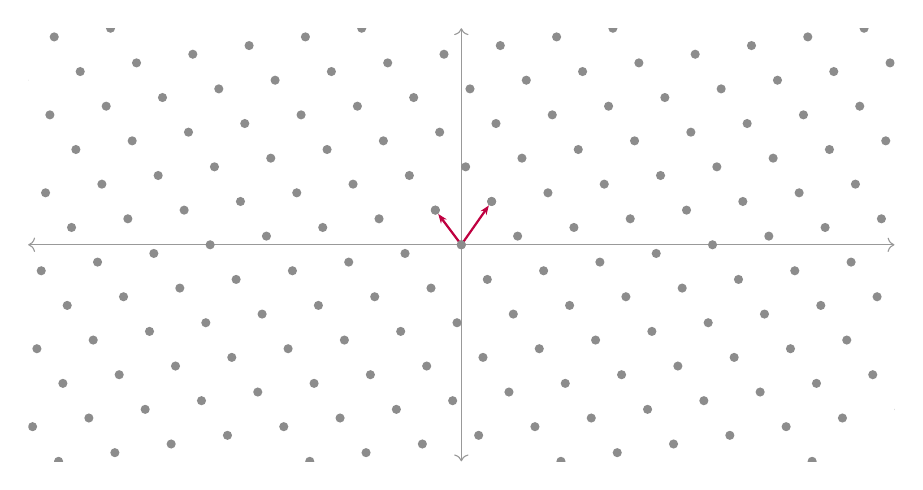
\begin{tikzpicture}
      \begin{scope}[scale=.55]
            \coordinate (Origin)   at (0,0);
            \coordinate (XAxisMin) at (-10,0);
            \coordinate (XAxisMax) at (10,0);
            \coordinate (YAxisMin) at (0,-5);
            \coordinate (YAxisMax) at (0,5);
            \draw [thin, black!40, <->] (XAxisMin) -- (XAxisMax);% Draw x axis
            \draw [thin, black!40,<->] (YAxisMin) -- (YAxisMax);% Draw y axis
            %\draw[style=help lines,dashed,black!20] (-5,-5) grid[step=1cm] (5,5);
    
            \begin{scope}
                \clip (-10,-5) rectangle (10,5); % Clips the picture...
                \pgftransformcm{1}{0.6}{0.7}{1}{\pgfpoint{0cm}{0cm}}
    
                % setup the nodes
                \foreach \x in {-20,...,20}
                \foreach \y in {-20,...,20}
                {
                  \node[shape=circle,fill=black!45,scale=0.35] (\x-\y) at (2*\x,\y+3){};
                }
            \end{scope}
    
            \node[shape=circle,fill=black!45,scale=0.35] (b1) at (-.6,.8){};
            \node[shape=circle,fill=black!45,scale=0.35] (b2) at (.7,1){};
            \draw [thick,purple,-{Stealth[length=1.2mm]}] (0,0) -- (b1);
            \draw [thick,purple,-{Stealth[length=1.2mm]}] (0,0) -- (b2);
            \node[shape=circle,fill=black!45,scale=0.35] at (0,0){};
    
        \end{scope}
    
      \end{tikzpicture}
  \end{figure}
\end{frame}

\begin{frame}{Name-dropping lattice problems}
  Some hard problems based on lattices
  \begin{itemize}[<+(1)->]
    \item Shortest vector problem
    \begin{itemize}
      \item Find the shortest non-zero vector
    \end{itemize}
    \item Closest vector problem
    \begin{itemize}
      \item Find a vector closest to a given vector
    \end{itemize}
    \item Shortest independent vectors problem
    \begin{itemize}
      \item Find a basis with the shortest vectors
    \end{itemize}
  \end{itemize}

  \pause
  Solving one solves the others
  \begin{itemize}[<+(1)->]
    \item Crypto usually does not use them directly
    \item The other problems are then shown to be equivalent in difficulty
  \end{itemize}
\end{frame}

\begin{frame}{Name-dropping LWE}
  Learning with errors (LWE) -- system of approximate equations
  \begin{itemize}[<+(1)->]
    \item Consider the linear equation system
    \[
      A \cdot s = b
    \]
    with $A \in \ZZ_q^{n \times m}$, $s\in\ZZ_q^m$, $b\in\ZZ_q^n$
    \item Add an error term $e\in\ZZ_q^n$ to obtain
    \[
      A \cdot s + e = b
    \]
    \item $s, e$ are secret, $A, b$ are public
    \item Variants exist: Ring-LWE, Module-LWE
  \end{itemize}
\end{frame}

\begin{frame}{NIST's PQC KEMs}
  ML-KEM (\href{https://csrc.nist.gov/pubs/fips/203/final}{FIPS 203}, CRYSTALS-Kyber)
    \begin{itemize}[<+(1)->]
      \item Primary KEM choice
      \item Based on the Module-LWE problem
      \item ML-KEM-512 ($\lambda = 128$), ML-KEM-768 ($\lambda = 192$), ML-KEM-1024 ($\lambda = 256$)
      \item Use at least ML-KEM-768, with ML-KEM-1024 sometimes required
    \end{itemize}

  \vspace*{1em}

  \pause
  HQC-KEM (will be FIPS 207, \href{https://www.nist.gov/news-events/news/2025/03/nist-selects-hqc-fifth-algorithm-post-quantum-encryption}{expected for 2027})
  \begin{itemize}[<+(1)->]
    \item Based on error-correcting codes
    \item Backup standard
  \end{itemize}
\end{frame}

\begin{frame}{NIST's PQC signature schemes}
  ML-DSA, \href{https://csrc.nist.gov/pubs/fips/204/final}{FIPS 204} (CRYSTALS-Dilithium)
  \pause
  \begin{itemize}
    \item Primary signature scheme choice
    \item Based on the Module-LWE problem
  \end{itemize}

  \vspace*{1em}

  \pause
  SLH-DSA, \href{https://csrc.nist.gov/pubs/fips/205/final}{FIPS 205} (SPHINCS+, hash-based backup)
  
  \vspace*{1em}

  \pause
  FIPS 206 will standardise FN-DSA (Falcon, NTRU-lattice-based)
\end{frame}

\begin{frame}{Alternatives}
  KEMs:
  \begin{itemize}
    \item FrodoKEM (lattices, LWE)
    \item Classic McEliece (code-based)
  \end{itemize}

  \vspace*{1em}

  \pause
  Stateful hash-based signature schemes (not recommended for general use)
  \begin{itemize}
    \item XMSS/XMSS\textsuperscript{MT}
    \item LMS/HSS
    \item Difficulty maintaining state
  \end{itemize}

  \vspace*{1em}

  \pause
  A good overview of the current standards is provided by \href{https://www.paloaltonetworks.com/cyberpedia/pqc-standards}{\textit{Palo Alto}}.
\end{frame}

\begin{frame}{Hybrid PQC}
  Hybrid mode: use classical and post-quantum algorithms simultaneously
  \begin{itemize}[<+(1)->]
    \item Do not confuse with \enquote{public-key + symmetric} hybrid
    \item For signing:
    \begin{itemize}
      \item Sign the message twice separately, then combine the signatures
      \item Separability issue: no single approach to fit all use cases
    \end{itemize}
    \item For key-exchange:
    \begin{itemize}
      \item Share two keys with a pre- and post-quantum KEX respectively
      \item Combine the shared secrets via KDF
    \end{itemize}
  \end{itemize}

  \pause
  Mostly recommended in EU, discouraged elsewhere (US, UK, Australia).
  \begin{itemize}
    \item Treat it as an interim approach
  \end{itemize}
\end{frame}

\begin{frame}{Crypto-agility}
  Algorithmic flexibility
  \begin{itemize}[<+(1)->]
    \item Application need not know which algorithm is used
    \item Algorithm \enquote{providers} for an application
    \item \enquote{No-regret move} to move towards crypto-agile systems
    \item Examples: X.509, TLS
  \end{itemize}
\end{frame}

\begin{frame}{Migration?}
  PQC is the future of cryptography, but when and how to migrate?
  \begin{itemize}[<+(1)->]
    \item Prioritise encryption (confidentiality cannot be extended in time)
    \item Hybrid (ANSSI, BSI) vs. not hybrid (NSA)
    \item Do something!
    \item \href{https://www.tno.nl/en/newsroom/2024/12/renewed-handbook-quantum-safe-crypto/}{\textit{PQC migration handbook}} (TNO)
  \end{itemize}

  \vspace*{1em}

  \pause
  New developments should all include PQC (or migration readiness)
  \begin{itemize}[<+(1)->]
    \item Crypto-agility and the existence of a cryptographic inventory (assets and algorithms) are the bare minimum
    \item Include these requirements in procurement documents (e.g. public sector)
  \end{itemize}
\end{frame}

\begin{frame}{PQC migration roadmap (simplified)}
  In the EU (mostly aligned with NIST), deadlines are as follows:
  \begin{itemize}[<+(1)->]
    \item By 31.12.2030, PQC transition completed for high-risk use cases
    \item By 31.12.2035, PQC transition completed for medium-risk use cases
    \item Prototypes and migration take time
    \item \href{https://digital-strategy.ec.europa.eu/en/library/coordinated-implementation-roadmap-transition-post-quantum-cryptography}{\textit{Roadmap for the Transition to Post-Quantum Cryptography}}
  \end{itemize}

  \vspace{1em}
  \pause
  Compliance will get you before the quantum computer does.
  Start early!
\end{frame}

\begin{frame}{PQC and TLS}
  TLS is the biggest PQC target
  \begin{itemize}[<+(1)->]
    \item \href{https://datatracker.ietf.org/doc/draft-ietf-tls-ecdhe-mlkem/}{X25519MLKEM768 (Draft)}
    \item \href{https://pq.cloudflareresearch.com}{\textit{Cloudflare on PQ key agreement}}
    \item (In Estonian) \href{https://www.ria.ee/blogi/tls-13-votme-kvantkindel-hubriidkehtestus-x25519mlkem768}{\textit{TLS 1.3 võtme kvantkindel hübriidkehtestus}} (RIA)
    \item \href{https://blog.cloudflare.com/kemtls-post-quantum-tls-without-signatures/}{KEM-TLS}
  \end{itemize}
\end{frame}

\begin{frame}{OpenSSL v. $\ge$3.5}
  Since v3.5, OpenSSL includes built-in support for ML-KEM, ML-DSA, SLH-DSA.
  \begin{itemize}[<+(1)->]
    \item Included with Ubuntu 26.04 LTS, released last month
    \item You get PQ-TLS for free
    \item For older versions, use the \href{https://openquantumsafe.org}{\textit{OQS provider}}
  \end{itemize}

  \vspace*{1em}

  \pause
  See also: \href{https://www.wolfssl.com/products/wolfcrypt-post-quantum/}{\textit{WolfSSL's PQC support}}
\end{frame}

\begin{frame}{Cryptographic Bill of Materials (CBOM)}
  Migration requires knowing what to migrate:
  \begin{itemize}[<+(1)->]
    \item Extension of SBOM (Software Bill of Materials)
    \item Representation of cryptographic assets within a system
    \begin{itemize}
      \item e.g. algorithms, keys, certificates
    \end{itemize}
  \end{itemize}

  \vspace*{1em}

  \pause
  Some guides/tooling:
  \begin{itemize}[<+(1)->]
    \item \href{https://cyclonedx.org/guides/OWASP_CycloneDX-Authoritative-Guide-to-CBOM-en.pdf}{\textit{Authoritative Guide to CBOM}} (OWASP)
    \item \href{https://www.nccoe.nist.gov/sites/default/files/2023-12/pqc-migration-nist-sp-1800-38b-preliminary-draft.pdf}{\textit{Migration to PQC Quantum Readiness: Cryptographic Discovery}} (NIST)
    \item \href{https://github.com/cbomkit}{CBOMkit} (\href{https://pqca.org}{PQC Alliance})
  \end{itemize}
\end{frame}

\begin{frame}{Quantum cryptography}
  Do not confuse post-quantum cryptography with quantum cryptography!

  \vspace*{1em}

  \pause
  Quantum cryptography:
  \begin{itemize}[<+(1)->]
    \item Uses properties of quantum physics for special constructions
    \item No computational hardness assumptions
    \item Quantum key distribution (QKD)
    \begin{itemize}
      \item Share a secret key over a quantum communication channel
      \item Eavesdropping becomes noticeable (the act of observing/measuring)
      \item Complex to implement and susceptible to DoS
    \end{itemize}
    \item Other crazy (but cool) constructions, e.g. mistrustful cryptography
  \end{itemize}
\end{frame}

\end{document}
